\documentclass [a4paper,11pt]{article}
\usepackage[T1]{fontenc}
\usepackage[utf8]{inputenc}
\usepackage[polish]{babel}
%\usepackage{amssymb}
\usepackage{amsthm}
\usepackage[intlimits]{amsmath}
\frenchspacing
\usepackage{indentfirst}
\usepackage{graphicx}
\usepackage{subfig}
\usepackage{mathptmx}
\usepackage{geometry}
\usepackage{wrapfig}
\usepackage{pdfpages}
\sloppy

\begin{document}
\newgeometry{tmargin=2cm, bmargin=2cm, lmargin=2cm, rmargin=2cm}

%----------- tabela nag?ówkowa---------------------- %
\begin{table}[]
\centering
\begin{tabular}{lllllll}
\cline{1-6}
\multicolumn{1}{|c|}{\begin{tabular}[c]{@{}c@{}}EAiIB\\ Informatyka\end{tabular}}              & \multicolumn{2}{l|}{\begin{tabular}[c]{@{}l@{}}Autor 1 Aleksander Lisiecki\\ Autor 2 Natalia Materek\end{tabular}}                                                                                                & \multicolumn{1}{c|}{\begin{tabular}[c]{@{}c@{}}Rok\\ II\end{tabular}}          & \multicolumn{1}{c|}{\begin{tabular}[c]{@{}c@{}}Grupa\\ II\end{tabular}}            & \multicolumn{1}{c|}{\begin{tabular}[c]{@{}c@{}}Zespół\\ VI\end{tabular}}      &  \\ \cline{1-6}
\multicolumn{1}{|c|}{\begin{tabular}[c]{@{}c@{}}Pracownia\\ FIZYCZNA\\ WFiIS AGH\end{tabular}} & \multicolumn{4}{l|}{\begin{tabular}[c]{@{}l@{}}Temat:\\ \textbf{Opracowanie danych pomiarowych} \end{tabular}}                                                                                                                                                                                                                                            & \multicolumn{1}{l|}{\begin{tabular}[c]{@{}l@{}}nr ćwiczenia:\\ 0\end{tabular}} &  \\ \cline{1-6}
\multicolumn{1}{|l|}{\begin{tabular}[c]{@{}c@{}}Data wykonania:\\ 3.12.2016\end{tabular}}      & \multicolumn{1}{c|}{\begin{tabular}[c]{@{}c@{}}Data oddania:\\ 7.12.2016\end{tabular}} & \multicolumn{1}{l|}{\begin{tabular}[c]{@{}l@{}}Zwrot do poprawki:\\ \phantom{data poprawki}\end{tabular}} & \multicolumn{1}{l|}{\begin{tabular}[c]{@{}l@{}}Data oddania:\\  \phantom{data oddania}\end{tabular}} & \multicolumn{1}{l|}{\begin{tabular}[c]{@{}l@{}}Data zaliczenia:\\  \phantom{data zaliczenia}\end{tabular}} & \multicolumn{1}{l|}{\begin{tabular}[c]{@{}l@{}}OCENA:\\ \phantom{ocena}\end{tabular}}       &  \\ \cline{1-6}
                                                                                               &                                                                                         &                                                                                     &                                                                                &                                                                                   &                                                                               & 
\end{tabular}
\end{table}

\section{Opis wahadła matematycznego }
\indent Wahadło matematyczne (wahadło proste) jest to ciało o masie punktowej $m$ zawieszone na cienkiej, nierozciągliwej nici o długości $l$. Kiedy ciało wytrącimy z równowagi, zaczyna się ono wahać w płaszczyźnie pionowej pod wpływem siły ciężkości. Jest to ruch okresowy.

\indent Jeśli wahadło wychylimy o niewielki kąt $\alpha$ to jego okres można wyrazić wzorem:
\begin{equation}
\label{wzor:okres}
 T= 2 \pi \sqrt{\frac{l}{g}} 
\end{equation}
gdzie
\begin{description}
\item [$T$] okres ruchu okresowego
\item [$l$] długość wahadła
\item [$g$] przyspieszenie ziemskie
\end{description}

\indent Przekształcając wzór {\ref{wzor:okres}} możemy wyznaczyć wartość przyspieszenia ziemskiego:

\begin{equation}
\label{wzor:przyspieszenie}
g= \frac{4 \pi^2 l}{T^2}
\end{equation}

\section{Opis układu pomiarowego}
\indent Badane wahadło przedstawione na rysunku {\ref{rys:1}} stanowi mosiężny obciążnik zawieszony na cienkiej lince. Linka jest podwieszona na
wolnostojącym statywie. Pomiary były dokonywane za pomocą stopera o dokładności 0,01 s. Do niepewności pomiaru stopera należy dodać czas reakcji osoby wykonującej pomiary, który został ustalony na $0,05 s$. 
Długość wahadła wyznaczono mierząc długość linki linijką o dokładności 1 mm. Na niepewność pomiaru długości wpływa oszacowanie odległości mocowania linki od środka obciążnika oraz trudność znalezienia punktu zawieszenia linki, została określona na 3 mm. Długość linki może być regulowana przez nawiniecie lub rozwiniecie linki na walec na którym jest umocowana.

\begin{figure}
\caption{Wahadlo schemat}
\label{rys:1}
\centering
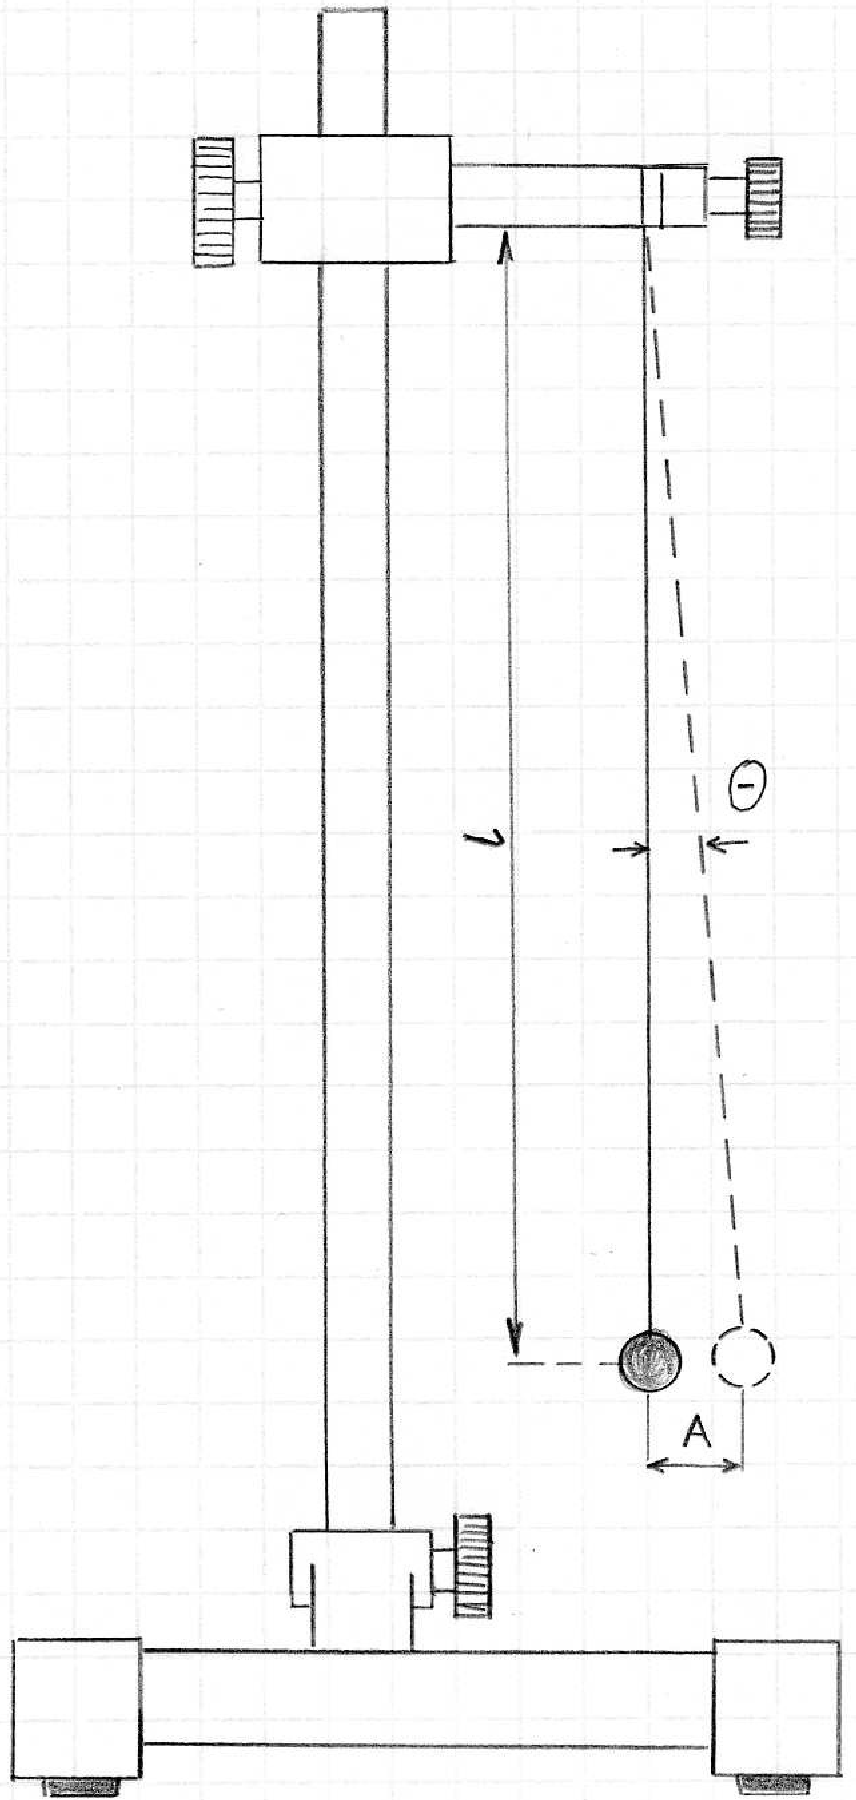
\includegraphics[width=0.3 \textwidth]{./wahadlo}
\end{figure}

\section{Etapy doświadczenia}
 \subsection{Wyznaczenie przyspieszenia ziemskiego korzystając z okresu drgań wahadła matematycznego:}
\begin{enumerate}
\item Zmierzenie długosci linki na której umocowany jest obciążnik
\item Wprawienie w ruch okresowy wahadła i włączenie stopera
\item Odczekanie aż wahadło wykona 15 pełnych okresów 
\item Zastopowanie stopera i zanotowanie wyniku
\item Powtórzenie czynności od 2 do 4 dziesięciokrotnie
\item Policzenie okresu dla pojedynczych prób (dzieląc wyniki przez 15)
\item Policzenie średniego okresu $T_{sr}$ korzystając z wyznaczonych okresów
\end{enumerate}

 \subsection{Badanie zależności okresu drgań od długości wahadła}
\indent W każdej próbie zmieniamy długość wahadła aby zaobserwować dla poszczególnych dŁugości różne okresy.
\begin{enumerate}
\item Zmienienie długości wahadła przez nawiniecie bądź rozwiniecie nitki na walec na którym jest mocowana
\item Wprawienie w ruch okresowy wahadła i włączenie stopera
\item Odczekanie aż wahadło wykona 15 pełnych okresów 
\item Zastopowanie stopera i zanotowanie wyniku
\item Policzenie okresu dla próby (dzieląc wyniki przez 15)  
\item Wróć do kroku 1
\indent Doświadczenie powtórzono dla czterech różnych długości wahadła.
\end{enumerate}

\section{Wyniki i ich opracowanie}
\subsection{Wyznaczanie wartości przyspieszenia ziemskiego}

\begin{table}[h!]
\centering
\caption{Wyniki pomiarów okresu drgań wahadła matematycznego}
\begin{tabular}{c|c|c}\hline

\label{table1}
$I[m]$ & $15*T[s]$ & $T[s])$\\ \hline
& 20,65 & 1,377 \\
& 19,97 & 1,331 \\
& 20,00 & 1,333 \\
& 19,85 & 1,323 \\
0,475 & 19,72 & 1,315 \\
& 20,26 & 1,351 \\
& 19,97 & 1,331 \\
& 20,25 & 1,350 \\
& 19,85 & 1,323 \\
& 20,30 & 1,353 \\ \hline
& $T_{\text{śr}}$ & 1,339 \\ \hline
\end{tabular}
\end{table}

\indent Wzór na wartość średnią okresu:
\begin{equation}
\label{wzor:okresSredni}
T_{\text{śr}}  = \frac{1}{n} \sum_{i=1}^{n} T_i
\end{equation}

gdzie
\begin{description}
\item [$T_{\text{śr}}$] średnia arytmetyczna $i$ okresów
\item [$T_{i}$] $i$- ty okres
\end{description}

\indent Wartość przyspieszenia ziemskiego:
\begin{equation}
\label{wzor:g}
g= \frac{4 \pi ^2 l}{ T_{\text{śr}}^2} = \frac{4 \cdot 3,141^2 \cdot 0,475} {1,339^2} \approx 10,.. \left[ \frac{m}{s^2} \right] 
\end{equation}

\subsection{Badanie zależności okresu drgań od długości wahadła}

\begin{table}[h!]
\centering
\caption{Wyniki pomiarów okresu drgań wahadła matematycznego w zależności od długości wahadła}
\begin{tabular}{c|c|c}\hline
\label{table2}
$I[m]$ & $15*T[s]$ & $T^{2}[s^{2}]$\\ \hline
0,475 & 20,65 & 1,896 \\
0,325 & 15,94 & 1,128 \\
0,355 & 17,00 & 1,284 \\
0,398 & 18,71 & 1,555 \\
0,240 & 13,93 & 0,8630 \\
0,195 & 13,06 & 0,7586 \\ \hline

\end{tabular}
\end{table}

Podnosząc wzór {\ref{wzor:okres}} na okres wahadła matematycznego obustronnie do kwadratu otrzymamy następującą zależność:
\begin{equation}
 T^2 = \frac{4 \pi^2}{g} \cdot l 
\end{equation}

\indent Konstruujemy wykres zależności $T^{2}$ od $l$. 
Wykres na rysunku{\ref{rys:2}} z linią regresji uzyskano przy pomocy funkcji REGLINP programu Excel. Widać że, wykres jest liniowy wiec można stwierdzić, ze proporcjonalnie do wzrostu długości wahadła $l$ rośnie kwadrat okresu wahadła $T^{2}$.
Dokładniej zwiększając długość wahadła dwukrotnie okres wahadła zwiększy się czterokrotnie.

\begin{figure}
\caption{Regresja liniowa}
\label{rys:2}
\centering
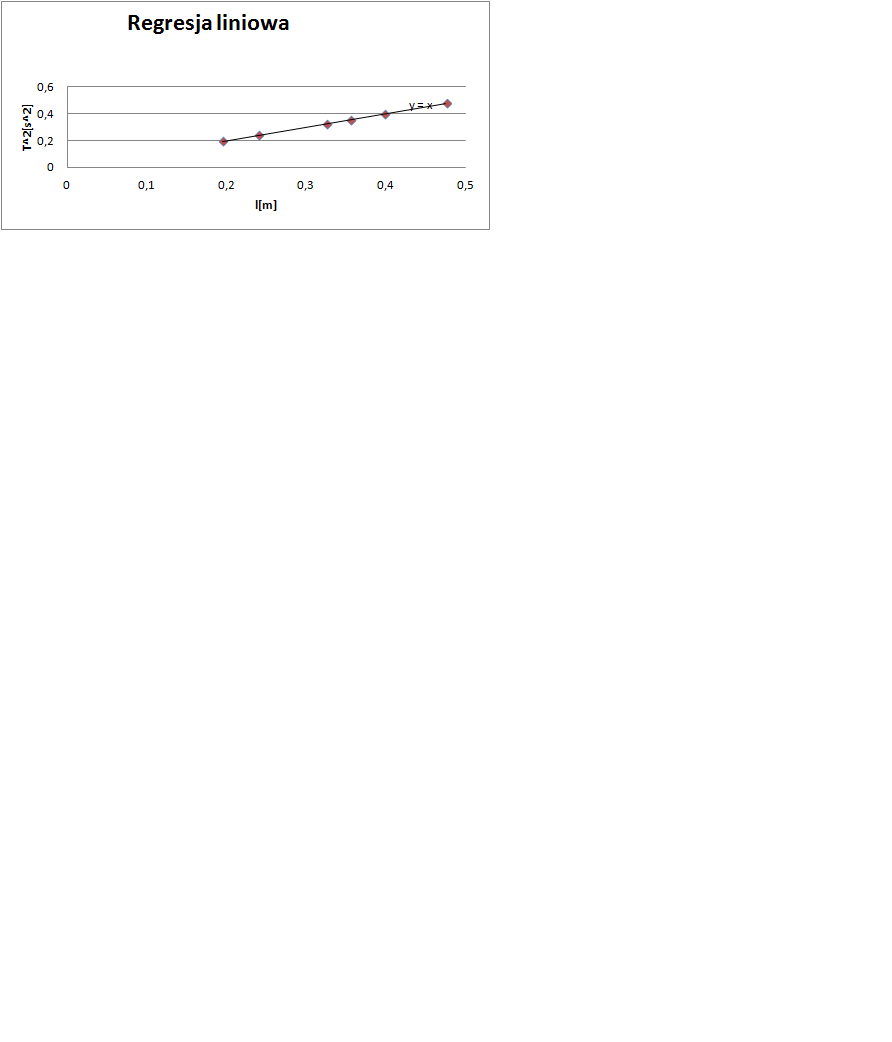
\includegraphics[width=1.2 \textwidth]{./wykres}
\end{figure}

\begin{table}[h!]
\centering
\caption{Wyniki uzyskane za pomocą funkcji REGLINP}
\begin{tabular}{c|c}\hline
\label{table2}
wartość $a$ & wartość $b$\\ 
27,79986 & 7,33731285  \\ \hline
niepewność wyznaczenia a & niepewność wyznaczenia b \\
1,435053 & 0,49410565 \\ \hline
współczynnik korelacji & niepewność wyznaczenia wartości y \\
0,989454 & 0,32916657 \\ \hline

\end{tabular}
\end{table}

\indent Współczynnik $a$ wynosi:
\begin{equation}
a = ...
\end{equation}

Znając współczynnik $a$ nachylenia wykresu możemy wyznaczyć przyspieszenie ziemskie $g$,
ponieważ: 
\begin{equation}
	T^2 = \frac{4 \pi^2}{g}\cdot l  
\end{equation} 
więc $g$:
\begin{equation}
	 a =   \frac{4 \pi^2}{g} \Longrightarrow g= \frac{4 \pi^2}{a}  \approx ... \left[ \frac{m}{s^2}\right]  
\end{equation}
	  

\newpage

\section{Szacowanie niepewności pomiarowych}
\subsection{Wyznaczanie wartości przyspieszenia ziemskiego}
\subsubsection{Niepewność pomiaru okresu}
\indent Posiadając serię pomiarów okresu wahadła dla tej samej długości, możemy obliczyć jego niepewność metodą typu A, czyli jako estymator odchylenia standardowego wielkości średniej:

\begin{equation}
u(T_{\text{śr}})  = \sqrt{\frac{\sum_{i=1}^{n} \left(T_i - T_{\text{śr}}\right)^2}{n(n-1)}} \approx ... [s]
\end{equation}  
gdzie
\begin{description}
\item [$u(T_{\text{śr}})$] niepewność okresu
\item [$T_{\text{śr}}$] okres wahadła
\item [$T_{i}$] $i$ -ty okres
\item [$n$] ilość prób 
\end{description}

\subsubsection{Niepewność pomiaru długości wahadła}
\indent Niepewność pomiaru długości jest szacowana metodą typu B na podstawie dokładności pomiaru:
\begin{equation}
u(l) = \frac{\Delta l}{\sqrt{3}} = \frac{0,003}{\sqrt{3}} \approx ... [m] 
\end{equation}
gdzie
\begin{description}
\item [$ \Delta l $] maksymalny błąd podczas mierzenia
\item [$u(l)$] niepewność długości
\end{description}

\subsubsection{Niepewność złożona pomiaru przyspieszenia ziemskiego}
\indent Przyspieszenie ziemskie jest wyznaczane pośrednio, wiec stosuje prawo przenoszenia niepewności:
\begin{equation}
u_c(g) = \sqrt{\left(  \frac{\delta g}{\delta T_{\text{śr}}} \right)^2 u(T_{\text{śr}})^2 + \left( \frac{\delta g}{\delta l} \right)^2 u(l)^2  } = \sqrt{\frac{64 \pi^4 l^2}{T_{\text{śr}}^6} u(T_{\text{śr}})^2 + \frac{16 \pi^4}{T_{\text{śr}}^4} u(l)^2}\approx ... \left[ \frac{m}{s^2} \right] 
\end{equation}
gdzie
\begin{description}
\item [$u_{c(g)}$] niepewność złożona przyspieszenia ziemskiego
\item [$ \frac{\delta g}{\delta T_{\text{śr}}} $] pochodna $g$ po $T_{\text{śr}}$
\item [$\frac{\delta g}{\delta l}$] pochodna $g$ po $l$
\end{description}

\indent Aby porównać wyznaczona wartość przyspieszenia ziemskiego z wartością tablicową obliczamy niepewność rozszerzoną:
\begin{equation}
	U_c(g) = k \cdot u_c(g) = 2 \cdot ... = ... \left[ \frac{m}{s^2} \right]
\end{equation} 
gdzie
\begin{description}
\item [$k$] współczynnik
\item [$U_c(g)$] niepewność rozszerzona
\end{description}

\indent Podsumowując wyznaczone przyspieszenie ziemskie ma wartość:
\begin{equation}
g = (... \pm ...)\left[ \frac{m}{s^2} \right]  
\end{equation}
 
\indent Wartość tablicowa przyspieszenia ziemskiego wynosi $g= 9,811 \left[ \frac{m}{s^2} \right] $ i  nie mieści się/mieści się w wyznaczonym przez nas przedziale.

\subsection{Badanie zależności okresu drgań od długości wahadła}
\indent Ponownie stosujemy prawo przenoszenia niepewności. Tym razem mamy do czynienia z funkcją jednej zmiennej: 
\begin{equation}
 g= \frac{4 \pi^2}{a}
\end{equation}

$$ u(g) = \frac{\delta g}{\delta a} u(a) =  - 4 \pi^2 a^{-2} \cdot u(a)$$

$$ |u(g)| =  4 \pi^2 a^{-2} \cdot u(a) \approx ...  \left[ \frac{m}{s^2}\right] $$

$$U_c(g) = k \cdot u_c(g) \approx 2 \cdot ... = ... \left[ \frac{m}{s^2} \right] $$

gdzie 
\begin{description}
\item [$a$] współczynnik nachylenia wykresu
\item [$u(g)$] niepewność $g$ uzyskanego na podstawie wykresu
\item [$u(a)$] niepewność współczynnika a (nachylenie wykresu)
\item [$\frac{\delta g}{\delta a}$] pochodna $g$ po $a$
\item [$u_{c(g)}$] niepewność złożona przyspieszenia ziemskiego
\item [$U_{c(g)}$] niepewność rozszerzona $g$
\end{description}
\indent Tak więc przyspieszenie ziemskie wyznaczone na podstawie wykresu zależności $T^2(l)$ ma wartość:
$$g = (... \pm ...)\left[ \frac{m}{s^2} \right] $$

\section{Podsumowanie doświadczenia}
\begin{table}[h!]
\begin{tabular}{|c|c|c|c|}
\hline Opis wielkości & Wynik $\left[ \frac{m}{s^2} \right]$ & u(g) $\left[ \frac{m}{s^2} \right]$ & $U_c(g)$ $\left[ \frac{m}{s^2} \right]$ \\
\hline $g$ za pomocą 10 pomiarów przy tej samej długości wahadła  & ... & ...  & ...  \\ 
\hline $g$ za pomocą wykresu $T^2(l)$ & ...  & ...  & ...  \\ 
\hline Wartość tablicowa $g$ & 9,811  & -  & -  \\ 
\hline 
\end{tabular} 
\end{table}

\section{Wnioski}
\begin{itemize}
\item Wyznaczenie przyspieszenia ziemskiego za pomocą wahadła matematycznego jest łatwym w wykonaniu doświadczeniem ale musimy liczyć się z niedokładnością pomiarów.
%\item Zakres uzyskanej warto?ci przyspieszenia ziemskiego wraz z niepewno?ci? uzyskanych za pomoc? %badania wykresu $T^2(l)$ zawiera w sobie warto?? tabelaryczn? przyspieszenia ziemskiego, a w przypadku %drugiej metody zakresy niepewno?ci mijaj? warto?? tabelaryczn? o bardzo ma?? warto??. ?wiadczy to o %poprawno?ci pomiarów
\item Jednym z powodów uzyskania różnych wartości przyspieszenia ziemskiego może być fakt że wahadło mogło się poruszać w więcej niż jednej płaszczyźnie.
\item Otrzymane wartości nie zgadzają się z wartościami tabelarycznymi i nie mieszczą się również w zakresie niepewności. Przyczyną błędu mogą być niewystarczająco dokładne przyrządy pomiarowe, niewykryty wcześniej błąd systematyczny np. związany opóźnieniem uruchamiania i zatrzymywania stopera lub zbyt duża amplituda z jaką wahał się ciężarek.  
\item Wraz z wydłużeniem nici, na której zawieszony jest ciężarek rośnie też okres wahadła. Tak jak zostało to przedstawione na wykresie {\ref{rys:2}}, zależność kwadratu okresu od długości wahadła jest zależnością proporcjonalną.
\end{itemize}

\end{document}